\section{Object 3}
\markright{Object 3}

The elbow body was formed with a swept feature guided along a curved path, and a square flange was extruded onto one end. Fillets were applied to the flange edges, and a circular pattern replicated a cut feature to produce the four bolt holes.

\begin{figure}[H]
	\centering

	\begin{subfigure}[b]{0.49\textwidth}
		\centering
		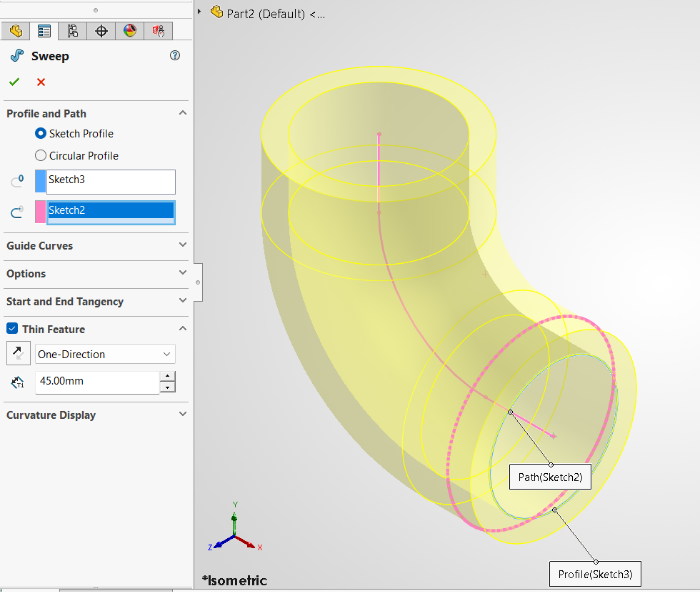
\includegraphics[width=\textwidth, keepaspectratio]{lab-02/assets/object-3/1.png}
		\caption{Sweep dialog with guide curve/path for the elbow body}
	\end{subfigure}%
	\hfill
	\begin{subfigure}[b]{0.49\textwidth}
		\centering
		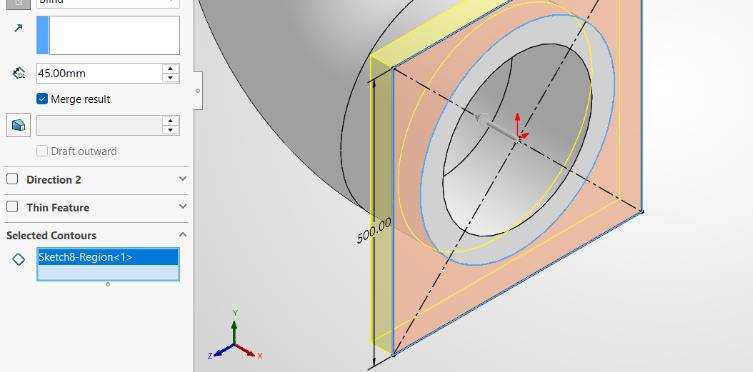
\includegraphics[width=\textwidth, keepaspectratio]{lab-02/assets/object-3/2.png}
		\caption{Extruding the flange}
	\end{subfigure}%
	\vspace{0.5em}
	\begin{subfigure}[b]{0.49\textwidth}
		\centering
		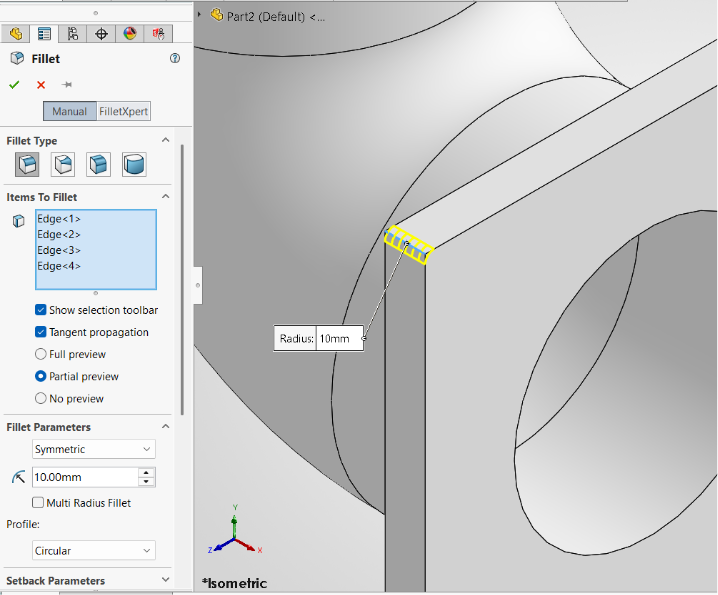
\includegraphics[width=\textwidth, keepaspectratio]{lab-02/assets/object-3/3.png}
		\caption{Applying fillets to the flange edges}
	\end{subfigure}%
	\hfill
	\begin{subfigure}[b]{0.49\textwidth}
		\centering
		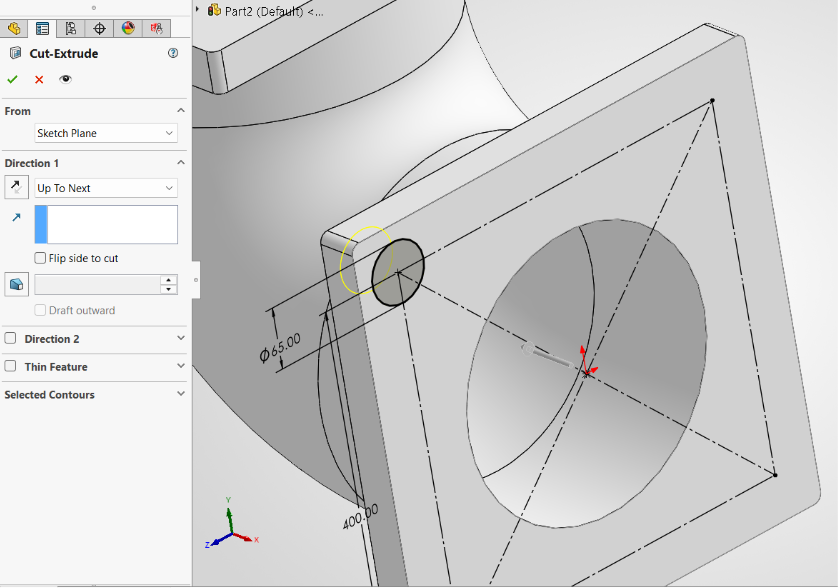
\includegraphics[width=\textwidth, keepaspectratio]{lab-02/assets/object-3/4.png}
		\caption{Circular pattern of the bolt holes}
	\end{subfigure}%
	\vspace{0.5em}
	\begin{subfigure}[b]{\textwidth}
		\centering
		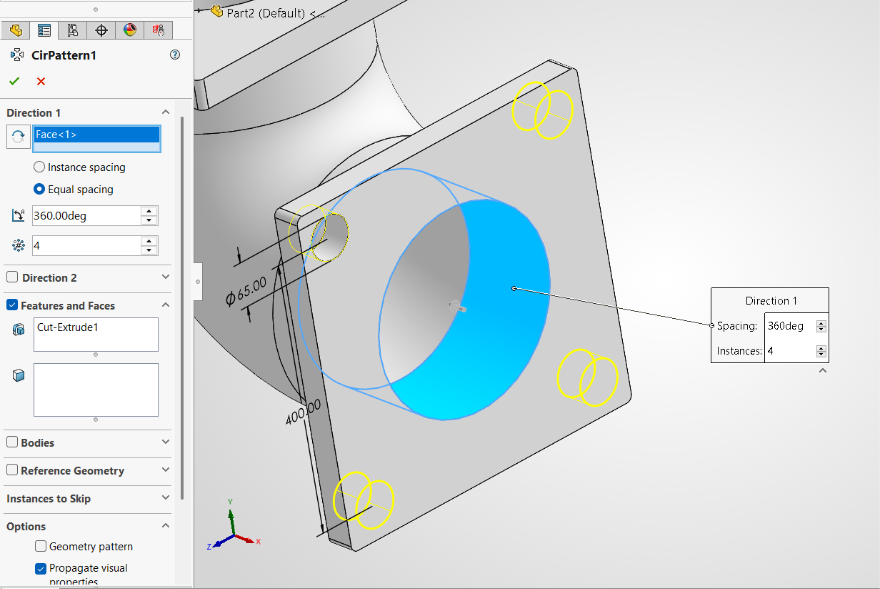
\includegraphics[width=\textwidth, keepaspectratio]{lab-02/assets/object-3/5.png}
		\caption{Final result}
	\end{subfigure}

	\caption{Snapshots while Designing Object 3 in Solidworks}
	\label{lab02_object_3}
\end{figure}
